

\tikzset{every picture/.style={line width=0.75pt}} %set default line width to 0.75pt        

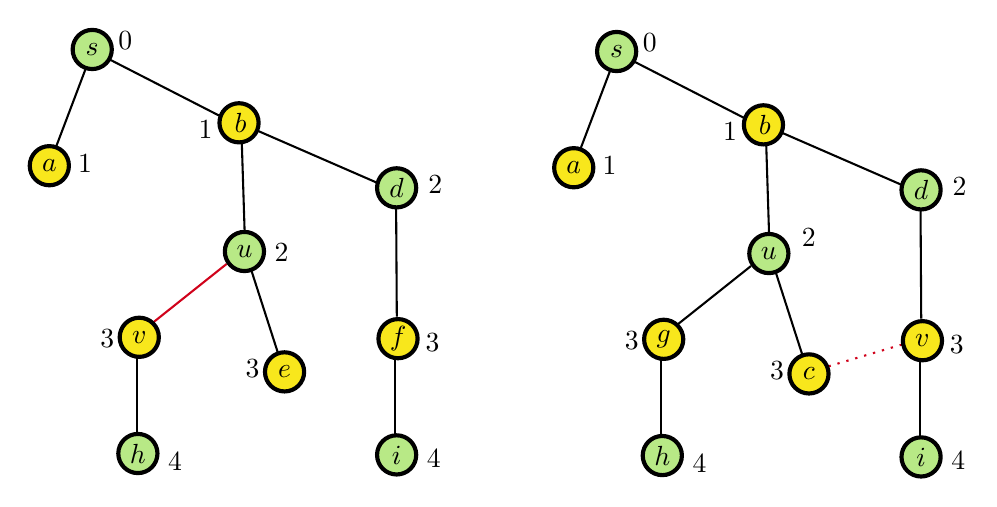
\begin{tikzpicture}[x=0.5pt,y=0.5pt,yscale=-1,xscale=1]
%uncomment if require: \path (0,376); %set diagram left start at 0, and has height of 376

%Straight Lines [id:da9915345378251853] 
\draw [color={rgb, 255:red, 0; green, 0; blue, 0 }  ,draw opacity=1 ][line width=0.75]    (70.5,53) -- (150.5,94) ;
%Straight Lines [id:da9064384352485415] 
\draw [color={rgb, 255:red, 0; green, 0; blue, 0 }  ,draw opacity=1 ][line width=0.75]    (263.5,142) -- (178.5,105) ;
%Straight Lines [id:da466470533029677] 
\draw [color={rgb, 255:red, 0; green, 0; blue, 0 }  ,draw opacity=1 ][line width=0.75]    (278,160) -- (278.5,239) ;
%Straight Lines [id:da3574505899142968] 
\draw [color={rgb, 255:red, 0; green, 0; blue, 0 }  ,draw opacity=1 ][line width=0.75]    (277.5,324) -- (277.5,270) ;
%Straight Lines [id:da5511077074666813] 
\draw [color={rgb, 255:red, 0; green, 0; blue, 0 }  ,draw opacity=1 ][line width=0.75]    (168.5,177) -- (166.5,114) ;
%Straight Lines [id:da31411403336049004] 
\draw [color={rgb, 255:red, 0; green, 0; blue, 0 }  ,draw opacity=1 ][line width=0.75]    (54,59) -- (32,117) ;
%Straight Lines [id:da30072725286752944] 
\draw [color={rgb, 255:red, 0; green, 0; blue, 0 }  ,draw opacity=1 ][line width=0.75]    (90.5,323) -- (90.5,269) ;
%Straight Lines [id:da17003523268457088] 
\draw [color={rgb, 255:red, 0; green, 0; blue, 0 }  ,draw opacity=1 ][line width=0.75]    (192.5,265) -- (173.5,206) ;
%Straight Lines [id:da48373225113468254] 
\draw [color={rgb, 255:red, 208; green, 2; blue, 27 }  ,draw opacity=1 ][line width=0.75]    (101.5,244) -- (155.5,201) ;
%Straight Lines [id:da2821401439481829] 
\draw [color={rgb, 255:red, 0; green, 0; blue, 0 }  ,draw opacity=1 ][line width=0.75]    (449.5,54.47) -- (529.5,95.47) ;
%Straight Lines [id:da6672632246558706] 
\draw [color={rgb, 255:red, 0; green, 0; blue, 0 }  ,draw opacity=1 ][line width=0.75]    (642.5,143.47) -- (557.5,106.47) ;
%Straight Lines [id:da32879840285784123] 
\draw [color={rgb, 255:red, 0; green, 0; blue, 0 }  ,draw opacity=1 ][line width=0.75]    (657,161.47) -- (657.5,240.47) ;
%Straight Lines [id:da43384321364795553] 
\draw [color={rgb, 255:red, 0; green, 0; blue, 0 }  ,draw opacity=1 ][line width=0.75]    (656.5,325.47) -- (656.5,271.47) ;
%Straight Lines [id:da5153233906529172] 
\draw [color={rgb, 255:red, 0; green, 0; blue, 0 }  ,draw opacity=1 ][line width=0.75]    (547.5,178.47) -- (545.5,115.47) ;
%Straight Lines [id:da37984064310004595] 
\draw [color={rgb, 255:red, 0; green, 0; blue, 0 }  ,draw opacity=1 ][line width=0.75]    (433,60.47) -- (411,118.47) ;
%Straight Lines [id:da9256177323063799] 
\draw [color={rgb, 255:red, 0; green, 0; blue, 0 }  ,draw opacity=1 ][line width=0.75]    (469.5,324.47) -- (469.5,270.47) ;
%Straight Lines [id:da20019335743654565] 
\draw [color={rgb, 255:red, 0; green, 0; blue, 0 }  ,draw opacity=1 ][line width=0.75]    (571.5,266.47) -- (552.5,207.47) ;
%Straight Lines [id:da9588741546915288] 
\draw [color={rgb, 255:red, 0; green, 0; blue, 0 }  ,draw opacity=1 ][line width=0.75]    (480.5,245.47) -- (534.5,202.47) ;
%Straight Lines [id:da5352595151461834] 
\draw [color={rgb, 255:red, 208; green, 2; blue, 27 }  ,draw opacity=1 ][line width=0.75]  [dash pattern={on 0.84pt off 2.51pt}]  (590.5,275) -- (644.5,259) ;

% Text Node
\draw  [fill={rgb, 255:red, 248; green, 231; blue, 28 }  ,fill opacity=1 ][line width=1.5]   (27.38, 130) circle [x radius= 14.15, y radius= 14.15]   ;
\draw (27.38,130) node   [align=left] {$\displaystyle a$};
% Text Node
\draw  [fill={rgb, 255:red, 184; green, 233; blue, 134 }  ,fill opacity=1 ][line width=1.5]   (58.38, 46) circle [x radius= 14.15, y radius= 14.15]   ;
\draw (58.38,46) node   [align=left] {$\displaystyle s$};
% Text Node
\draw  [fill={rgb, 255:red, 248; green, 231; blue, 28 }  ,fill opacity=1 ][line width=1.5]   (164.48, 99) circle [x radius= 14.15, y radius= 14.15]   ;
\draw (158.98,99) node [anchor=west] [inner sep=0.75pt]   [align=left] {$\displaystyle b$};
% Text Node
\draw  [fill={rgb, 255:red, 184; green, 233; blue, 134 }  ,fill opacity=1 ][line width=1.5]   (168.38, 192) circle [x radius= 14.15, y radius= 14.15]   ;
\draw (168.38,192) node   [align=left] {$\displaystyle u$};
% Text Node
\draw  [fill={rgb, 255:red, 184; green, 233; blue, 134 }  ,fill opacity=1 ][line width=1.5]   (278.38, 146) circle [x radius= 14.15, y radius= 14.15]   ;
\draw (278.38,146) node   [align=left] {$\displaystyle d$};
% Text Node
\draw  [fill={rgb, 255:red, 184; green, 233; blue, 134 }  ,fill opacity=1 ][line width=1.5]   (278.38, 339) circle [x radius= 14.15, y radius= 14.15]   ;
\draw (278.38,339) node   [align=left] {$\displaystyle i$};
% Text Node
\draw  [fill={rgb, 255:red, 248; green, 231; blue, 28 }  ,fill opacity=1 ][line width=1.5]   (279.38, 255) circle [x radius= 14.15, y radius= 14.15]   ;
\draw (279.38,255) node   [align=left] {$\displaystyle f$};
% Text Node
\draw  [fill={rgb, 255:red, 184; green, 233; blue, 134 }  ,fill opacity=1 ][line width=1.5]   (91.38, 338) circle [x radius= 14.15, y radius= 14.15]   ;
\draw (91.38,338) node   [align=left] {$\displaystyle h$};
% Text Node
\draw  [fill={rgb, 255:red, 248; green, 231; blue, 28 }  ,fill opacity=1 ][line width=1.5]   (92.38, 254) circle [x radius= 14.15, y radius= 14.15]   ;
\draw (92.38,254) node   [align=left] {$\displaystyle v$};
% Text Node
\draw  [fill={rgb, 255:red, 248; green, 231; blue, 28 }  ,fill opacity=1 ][line width=1.5]   (197.38, 279) circle [x radius= 14.15, y radius= 14.15]   ;
\draw (197.38,279) node   [align=left] {$\displaystyle e$};
% Text Node
\draw (75,31) node [anchor=north west][inner sep=0.75pt]   [align=left] {$\displaystyle 0$};
% Text Node
\draw (46,120) node [anchor=north west][inner sep=0.75pt]   [align=left] {$\displaystyle 1$};
% Text Node
\draw (133,95) node [anchor=north west][inner sep=0.75pt]   [align=left] {$\displaystyle 1$};
% Text Node
\draw (188,184) node [anchor=north west][inner sep=0.75pt]   [align=left] {$\displaystyle 2$};
% Text Node
\draw (62,246) node [anchor=north west][inner sep=0.75pt]   [align=left] {$\displaystyle 3$};
% Text Node
\draw (167,268) node [anchor=north west][inner sep=0.75pt]   [align=left] {$\displaystyle 3$};
% Text Node
\draw (111,335) node [anchor=north west][inner sep=0.75pt]   [align=left] {$\displaystyle 4$};
% Text Node
\draw (298,333) node [anchor=north west][inner sep=0.75pt]   [align=left] {$\displaystyle 4$};
% Text Node
\draw (297,249) node [anchor=north west][inner sep=0.75pt]   [align=left] {$\displaystyle 3$};
% Text Node
\draw (299,135) node [anchor=north west][inner sep=0.75pt]   [align=left] {$\displaystyle 2$};
% Text Node
\draw  [fill={rgb, 255:red, 248; green, 231; blue, 28 }  ,fill opacity=1 ][line width=1.5]   (406.38, 131.47) circle [x radius= 14.15, y radius= 14.15]   ;
\draw (406.38,131.47) node   [align=left] {$\displaystyle a$};
% Text Node
\draw  [fill={rgb, 255:red, 184; green, 233; blue, 134 }  ,fill opacity=1 ][line width=1.5]   (437.38, 47.47) circle [x radius= 14.15, y radius= 14.15]   ;
\draw (437.38,47.47) node   [align=left] {$\displaystyle s$};
% Text Node
\draw  [fill={rgb, 255:red, 248; green, 231; blue, 28 }  ,fill opacity=1 ][line width=1.5]   (543.48, 100.47) circle [x radius= 14.15, y radius= 14.15]   ;
\draw (537.98,100.47) node [anchor=west] [inner sep=0.75pt]   [align=left] {$\displaystyle b$};
% Text Node
\draw  [fill={rgb, 255:red, 184; green, 233; blue, 134 }  ,fill opacity=1 ][line width=1.5]   (547.38, 193.47) circle [x radius= 14.15, y radius= 14.15]   ;
\draw (547.38,193.47) node   [align=left] {$\displaystyle u$};
% Text Node
\draw  [fill={rgb, 255:red, 184; green, 233; blue, 134 }  ,fill opacity=1 ][line width=1.5]   (657.38, 147.47) circle [x radius= 14.15, y radius= 14.15]   ;
\draw (657.38,147.47) node   [align=left] {$\displaystyle d$};
% Text Node
\draw  [fill={rgb, 255:red, 184; green, 233; blue, 134 }  ,fill opacity=1 ][line width=1.5]   (657.38, 340.47) circle [x radius= 14.15, y radius= 14.15]   ;
\draw (657.38,340.47) node   [align=left] {$\displaystyle i$};
% Text Node
\draw  [fill={rgb, 255:red, 248; green, 231; blue, 28 }  ,fill opacity=1 ][line width=1.5]   (658.38, 256.47) circle [x radius= 14.15, y radius= 14.15]   ;
\draw (658.38,256.47) node   [align=left] {$\displaystyle v$};
% Text Node
\draw  [fill={rgb, 255:red, 184; green, 233; blue, 134 }  ,fill opacity=1 ][line width=1.5]   (470.38, 339.47) circle [x radius= 14.15, y radius= 14.15]   ;
\draw (470.38,339.47) node   [align=left] {$\displaystyle h$};
% Text Node
\draw  [fill={rgb, 255:red, 248; green, 231; blue, 28 }  ,fill opacity=1 ][line width=1.5]   (471.38, 255.47) circle [x radius= 14.15, y radius= 14.15]   ;
\draw (471.38,255.47) node   [align=left] {$\displaystyle g$};
% Text Node
\draw  [fill={rgb, 255:red, 248; green, 231; blue, 28 }  ,fill opacity=1 ][line width=1.5]   (576.38, 280.47) circle [x radius= 14.15, y radius= 14.15]   ;
\draw (576.38,280.47) node   [align=left] {$\displaystyle c$};
% Text Node
\draw (454,32.47) node [anchor=north west][inner sep=0.75pt]   [align=left] {$\displaystyle 0$};
% Text Node
\draw (425,121.47) node [anchor=north west][inner sep=0.75pt]   [align=left] {$\displaystyle 1$};
% Text Node
\draw (512,96.47) node [anchor=north west][inner sep=0.75pt]   [align=left] {$\displaystyle 1$};
% Text Node
\draw (569,173.47) node [anchor=north west][inner sep=0.75pt]   [align=left] {$\displaystyle 2$};
% Text Node
\draw (441,247.47) node [anchor=north west][inner sep=0.75pt]   [align=left] {$\displaystyle 3$};
% Text Node
\draw (546,269.47) node [anchor=north west][inner sep=0.75pt]   [align=left] {$\displaystyle 3$};
% Text Node
\draw (490,336.47) node [anchor=north west][inner sep=0.75pt]   [align=left] {$\displaystyle 4$};
% Text Node
\draw (677,334.47) node [anchor=north west][inner sep=0.75pt]   [align=left] {$\displaystyle 4$};
% Text Node
\draw (676,250.47) node [anchor=north west][inner sep=0.75pt]   [align=left] {$\displaystyle 3$};
% Text Node
\draw (678,136.47) node [anchor=north west][inner sep=0.75pt]   [align=left] {$\displaystyle 2$};


\end{tikzpicture}

